\documentclass{ximera}

\newcommand{\RR}{\mathbb R}
\renewcommand{\d}{\,d}
\newcommand{\dd}[2][]{\frac{d #1}{d #2}}
\renewcommand{\l}{\ell}
\newcommand{\ddx}{\frac{d}{dx}}
\newcommand{\dfn}{\textbf}
\newcommand{\eval}[1]{\bigg[ #1 \bigg]}


\outcome{Determine if a series converges using the alternating series test.}

\title[Dig-In:]{remainders for alternating series}
\author{Jim Talamo}

\begin{document}
\begin{abstract}
There is a nice result for approximating the remainder of convergent alternating series. 
\end{abstract}
\maketitle

\section{Introduction}
Recall that if $\{a_n\}_{n=n_0}$ is a sequence of positive terms, we say that $\sum_{k=n_0}^{\infty}$ is an alternating series, and we have a nice result to test these for convergence, which is reprinted below.

\begin{theorem}[Alternating Series Test]
Let $\{a_n\}$ be a sequence whose terms are eventually positive and nonincreasing and
$\lim_{n\to\infty}a_n=0$. Then, the series 
\[
\sum_{n=1}^\infty (-1)^{n}a_n \qquad \text{and}\qquad \sum_{n=1}^\infty (-1)^{n+1}a_n 
\]
both converge.
\end{theorem}


Note that this test gives us a way to determine if many alternating series \emph{must} converge, but it does not give us information about the value to which the series converges.  If we want to obtain insight as to what the approximate value of the convergent series is, we must study remainders.

  


%%%%%%%%%%%%%%%%%%%%%%%%%%%%%%%%%%%%%%%%%%%%%%%%%%%%%%%%%%%%%%%%%%%%%%

\section{Remainders for Alternating Series}
As usual we must establish that a series converges first before we begin to think about remainders.  Once we have established that an alternating series $\sum_{k=1}^{\infty} (-1)^k a_k$ converges, we recall the important result

\begin{image}
  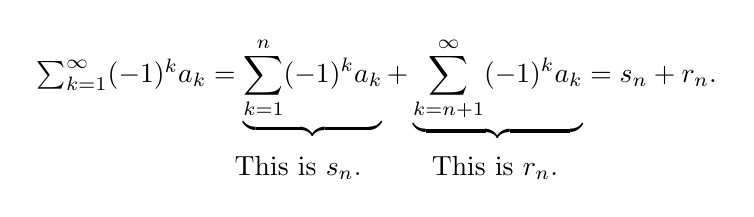
\begin{tikzpicture}
        \node at (0,0) {
          $ \sum_{k=1}^{\infty} (-1)^k a_k=\underbrace{\sum_{k=1}^{n}(-1)^k a_k}+ \underbrace{\sum_{k=n+1}^\infty (-1)^k a_k} = s_n+r_n$.};
        \node at (1.5,-1) { This is $r_n$.};
       
        \node at (-1,-1) { This is $s_n$. };
        
      \end{tikzpicture}
  \end{image}

While we cannot find an explicit formula for $s_n$ here.  As such, if we want to establish a good estimate, we will need to approximate the infinite sum by a term in the sequence of partial sums and try to establish an error estimate.  Thankfully, we have such an estimate.



\begin{theorem}[Alternating Series Remainder Estimates]\index{alternating series remainder estimates}
Let $\{a_n\}_{n=n_0}$ be a sequence whose terms are positive and nonincreasing  and
$\lim_{n\to\infty}a_n=0$. Then,  
\[
\big| r_n \big| \leq a_{n+1} \qquad \textrm{ for all } n \geq n_0.
\]
\end{theorem}

Note that the above guarantees that for any integer $N>n_0$, the term $s_N$ will approximate the series $\sum_{k=1}^{\infty} a_k$ with an error no greater than $a_{n+1}$.  Before we work an example, a few comments are in order.

\begin{itemize}
\item[1.] In most cases, we will have $n_0 = 0$ or $n_0 =1$.  As a technical point, we have to make the specification of when the sequence $\{a_n\}$ is actually both nonincreasing and contains only positive terms before we can use the result.  
\item[2.] If the sequence $\{a_n\}_{n = n_0}$ meets the criteria, note that we can split up the series $\sum_{k=1}^{\infty} a_k$ as 

\[ 
\sum_{k=1}^{\infty} a_k = \sum_{k=1}^{n_0} a_k +\sum_{k=n_0+1}^{\infty} a_k 
\]

We can compute the first sum by hand since it requires adding finitely many terms, then use the remainder result on the infinite series.
\end{itemize}



\begin{example}
Consider the alternating geometric series $\sum_{k=0}^{\infty} (-1)^k \left(\frac{1}{2}\right)^k$.

\begin{itemize}
\item[I.] Compute $\sum_{k=0}^{\infty} (-1)^k \left(\frac{1}{2}\right)^k$.
\item[II.] Use the theorem above to obtain an estimate for the remainder if $s_4$ is used to approximate the series.  What do you notice?
\end{itemize}

\begin{explanation}
First, note that by using laws of exponents, $\sum_{k=0}^{\infty} (-1)^k \left(\frac{1}{2}\right)^k = \sum_{k=0}^{\infty}  \left(\frac{-1}{2}\right)^k$.   

the geometric series $\sum_{k=0}^{\infty} (-1)^k \left(\frac{1}{2}\right)^k$ converges because $|r| = \frac{1}{2} <1$.

\begin{itemize}
\item[I.] When $r<1$, note that $\sum_{k=0}^{\infty} ar^k = \frac{a}{1-r}$.  Here, $r= -\frac{1}{2}$, so we find that $\sum_{k=0}^{\infty} (-1)^k \left(\frac{1}{2}\right)^k= \frac{2}{3}.$
\item[II.] Since $\left\{\left(\frac{1}{2}\right)^k\right\}_{k=0}$ is decreasing and $\lim_{n \to \infty} \left(\frac{1}{2}\right)^n =0$, we can use the remainder results.  If we use $s_7$ to approximate  $\sum_{k=0}^{\infty} (-1)^k \left(\frac{1}{2}\right)^k$, we have $n=7$, and conclude

\[
|r_4| < a_5 = \left(\frac{1}{2}\right)^5 = \frac{1}{32}.
\]

We can explicitly compute $s_4$ by using the formula for partial sums for geometric series or by hand.

\[
s_4 = 1-\frac{1}{2}+\frac{1}{4}-\frac{1}{8}+\frac{1}{16} = \frac{11}{16}.
\]

We note that to five decimal places, we have the following.

\begin{itemize}
\item The error bound from the theorem is $|r_4| < \frac{1}{32} = .03125$.
\item The approximate value of the series $\sum_{k=0}^{\infty} (-1)^k \left(\frac{1}{2}\right)^k$ is $s_4 = \frac{11}{16} = .68750$.
\item The actual value of the series $\sum_{k=0}^{\infty} (-1)^k \left(\frac{1}{2}\right)^k$ is $\frac{2}{3} \approx .66667$.
\end{itemize}

Thus, $s_4$ is actually within $.02083$ of the actual value of $\sum_{k=0}^{\infty} (-1)^k \left(\frac{1}{2}\right)^k$; $s_4$ is thus within the $.03125$ of the actual value of $\sum_{k=0}^{\infty} (-1)^k \left(\frac{1}{2}\right)^k$ guaranteed by the remainder result.

\end{itemize}
\end{explanation}
\end{example}

In the above example, we could compute the exact value of the series in question, so the remainder result could be verified explicitly.  In the next example, the exact value of the series is not known, but we can approximate as closely as we want.

\begin{example}
Consider the alternating series $\sum_{k=1}^{\infty} \frac{(-1)^k}{k^3}$.

\begin{itemize}
\item[I.] Find a value for $N$ so $s_N$ approximates $\sum_{k=1}^{\infty} \frac{(-1)^k}{k^3}$ to within $.0001$ of its actual value.
\item[II.] Using technology, compute $\sum_{k=1}^{\infty} \frac{(-1)^k}{k^3}$ to within $.0001$.
\item[III.] Using technology, it can be shown that $\sum_{k=1}^{100000} \frac{(-1)^k}{k^3} = -.9015426774$ to ten decimal places.  Using the remainder result, how far off from the exact value of the series $\sum_{k=1}^{100000} \frac{(-1)^k}{k^3}$ could this be?
\end{itemize}

\begin{explanation}
Check for yourself that $\sum_{k=1}^{\infty} \frac{(-1)^k}{k^3}$ satisfies the criteria for the remainder result for alternating series to hold before reading on.

\begin{itemize}
\item[I.] To find a value for $N$ so $s_N$ approximates $\sum_{k=1}^{\infty} \frac{(-1)^k}{k^3}$ to within $.0001$ of its actual value, we can find $N$ so $\big|r_N\big| < .0001$.  Since we have an explicit formula $a_n = \frac{1}{n^3}$ and that $\big|r_N\big| < a_{N+1}$, we can set $a_{N+1} < .0001$ (so $|r_N|$ will be less than $.0001$ by transitivity).

\begin{align*}
a_{N+1} = \frac{1}{\answer{\left(N+1\right)^3}} &< .0001 \\
1 &<  .0001 (N+1)^3 \\
\answer{10000} &< (N+1)^3 \\
21.54 &< N+1 \qquad  \textrm{ (to two decimal places) }\\
20.54 &< N \\
\end{align*}

We should thus use $N =$  \wordChoice{\choice{$20$}\choice[correct]{$21$}}.

\item[II.] We can thus approximate $\sum_{k=1}^{\infty} \frac{(-1)^k}{k^3}$ by using \wordChoice{\choice{$s_20$}\choice[correct]{$s_21$}}.  While this would be tedious to do by hand, technology can compute this sum quickly to find 

\[
\sum_{k=1}^{21} \frac{(-1)^k}{k^3} \approx -.90159.
\]

Using this result above, we conclude that $-.90159-.0001 \leq \sum_{k=1}^{\infty} \frac{(-1)^k}{k^3} \leq -.90159+.0001$ or

\[
-.90169 \leq \sum_{k=1}^{\infty} \frac{(-1)^k}{k^3} \leq -.90149
\]
\item[III.] Here, we have used $s_{100000}$ to approximate the value of the series.  The remainder result tells us that the error $r_{100000}$ made in this approximation can be no worse than $a_{100001}$; i.e.

\[
\big|r_{100000}\big| < \frac{1}{(100001)^3}. 
\]

Noting that $\frac{1}{(100001)^3} = 9.9997 \times 10^{-16}$, we see that the approximation given above corresponds with the actual value of the series to the ten decimal places listed.

\end{itemize}
\end{explanation}
\end{example}




\end{document}
